\documentclass[11pt]{article}

\usepackage{centernot}
\usepackage{amssymb}
\usepackage{xcolor}
\definecolor{myblue}{RGB}{0, 0, 255} 
\definecolor{mygreen}{RGB}{0, 180, 80}
\definecolor{myred}{RGB}{153, 0, 0}
\definecolor{myorange}{RGB}{255, 153, 51}
\definecolor{mypurple}{RGB}{102, 0, 204}
\usepackage{verbatim}
\usepackage{multicol}
\usepackage{enumitem}
\usepackage{amsfonts}
\usepackage{amsmath}
\usepackage[utf8]{inputenc}
\usepackage[export]{adjustbox}  % for correct logo rendering
\usepackage{fancyhdr}  % for header/footer formatting
\usepackage{hyperref}  % for hyper-references
\usepackage{datetime}  % to update month in footer
\usepackage{array}  % more flexible tables
\usepackage[includeheadfoot,
            left=1in,
            right=1in,
            top=0.75in,
            bottom=0.75in,
            headheight=40pt]{geometry} % geometry needs to know headheight to correctly render the footer
\usepackage{tikz} % For drawing grid boxes

\definecolor{darkblue}{RGB}{0, 0, 139}
\definecolor{lightblue}{RGB}{173, 216, 230}

% desired format for footer
\newdateformat{monthyeardate}{%
  \monthname[\THEMONTH] \THEYEAR}

% set up header/footer
\pagestyle{fancy}
\fancyhf{}  % clear all headers/footers
\renewcommand{\headrulewidth}{0pt}  % remove header rule
\renewcommand{\footrulewidth}{0pt}  % remove footer rule

% set up header

\fancypagestyle{firstpage}{
    \fancyhead[L]{
    \vspace{0pt}
    \hspace{-8pt}
    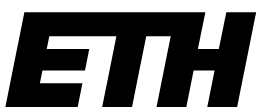
\includegraphics[width=0.1\textwidth]{docimgs/eth_logo_kurz_pos.png}\\
    \textbf{Swiss Federal Institute of Technology}\\
    \textbf{Zurich}\\
    %\textbf{ } \\
    
    }    

    \fancyhead[R]{
    \raggedleft
    %\vspace{20pt}
    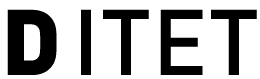
\includegraphics[width=0.13\textwidth]{docimgs/eth_ditet_logo_pos.png}\\
     \textbf{Dept. of Information Technology and} \\ \textbf{Electrical Engineering}  \\
     %\textbf{Chair for Mathematical Information} \\ \textbf{Information Science} \\

    }
}

% set up footer
\fancyfoot[L]{mdietz, ÜS 7}
\fancyfoot[C]{\thepage}
\fancyfoot[R]{\monthyeardate\today}

% set up section/subsection titles
\renewcommand{\thesection}{\arabic{section}}
\renewcommand{\thesubsection}{\arabic{subsection}}

% command used for simply emphasizing suggestions
\newcommand{\suggestion}[1]{{\itshape #1}}

%--- commands for transform arrows----------------
\newcommand{\transform}[2]{%
    \begin{tikzpicture}
        % Open circle
        \draw[thick] (0,0) circle (0.1);
        % Line with number above and adjustable length
        \draw[thick] (0.1,0) -- (#2,0) node[midway, above] {#1};
        % Filled circle
        \filldraw[thick] (#2,0) circle (0.1);
    \end{tikzpicture}%
}
\newcommand{\invtransform}[2]{%
    \begin{tikzpicture}
        % filled circle
        \filldraw[thick] (0,0) circle (0.1);
        % Line with number above and adjustable length
        \draw[thick] (0.1,0) -- (#2 -0.1,0) node[midway, above] {#1};
        % open circle
        \draw[thick] (#2,0) circle (0.1);
    \end{tikzpicture}%
}
\newcommand{\verticaltransform}[4]{%
    \begin{tikzpicture}
        % Open circle at the bottom with text below
        \filldraw[thick] (0,0) circle (0.1) node[below=3pt] {$#4$};
        % Vertical line with number on the left
        \draw[thick] (0,0.1) -- (0,#2 -0.1) node[midway, left] {#1};
        % Filled circle at the top with text above
        \draw[thick] (0,#2) circle (0.1) node[above=3pt] {$#3$};
    \end{tikzpicture}%
}
\newcommand{\verticalinvtransform}[4]{%
    \begin{tikzpicture}
        % Open circle at the bottom with text below
        \draw[thick] (0,0) circle (0.1) node[below=3pt] {$#4$};
        % Vertical line with number on the left
        \draw[thick] (0,0.1) -- (0,#2) node[midway, left] {#1};
        % Filled circle at the top with text above
        \filldraw[thick] (0,#2) circle (0.1) node[above=3pt] {$#3$};
    \end{tikzpicture}%
}

\begin{document}
\thispagestyle{firstpage}

\setlength{\headheight}{1 \baselineskip}  % accomodate header
\setlength{\parindent}{0pt}  % remove initial paragraph indent
\setlength{\parskip}{\baselineskip}  % add skip between paragraphs

\vspace*{-5px}
\section*{Übungsstunde 7}

\section*{Themenüberblick}
\begin{itemize}
    \item \textbf{Spezielle Eingangssignale von LTI-Systemen}
    \item[] Repetition: Fourierreihen
    \item[] Plancherel und Parseval für periodische Signale
    \item \textbf{Anwendungen der Fouriertransformation auf LTI-Systeme}
    \item[] Ideale Tiefpassfilter
    \item[] Bandbegrenzte Signale
\end{itemize}

\section*{Aufgaben für diese Woche}
\vspace{-0.5cm}

\textbf{67}, \textbf{68}, 69, \textbf{70}, 71, \textbf{72}, 73, 74, 75, \textbf{76}, \textbf{77}\\
\vspace{-0.5cm}

69-74 waren schon letze Woche dabei.\\
\vspace{-0.5cm}

Die \textbf{fettgedruckten} Übungen empfehle ich, weil sie wesentlich zu eurem Verständnis der Theorie beitragen und/oder sehr prüfungsrelevant sind.

\vfill \null
\pagebreak

\section*{Repetition: Fourierreihen}
\vspace*{-0.5cm}
\begin{itemize}[leftmargin=0pt]
    \item[] Für $T-$periodische Signale $x(t)$ gilt:
    \item[] \fcolorbox{darkblue}{lightblue}{%
    \parbox{\dimexpr\linewidth-2\fboxsep-2\fboxrule\relax}{
        $$x(t) = x(t + T) = \sum_{k=-\infty}^{\infty} c_k e^{\frac{2 \pi i k t}{T}}, \hspace{12pt} \text{wobei} \hspace{12pt} c_k = \frac{1}{T}\int_0^T x(t) e^{-\frac{2 \pi i k t}{T}} \text{d}t \hspace{12pt} \forall k \in \mathbb{Z}$$
        \hspace{33pt} Gemäss Nr. 21 aus der Formelsammlung wird dieses $x(t)$ fouriertransformiert zu:
        $$(\mathcal{F}x)(f) = \hat{x}(f) = \mathcal{F}\left\{ \sum_{k = -\infty}^{\infty} c_k e^{\frac{2 \pi i k t}{T}}\right\} = \sum_{k = -\infty}^{\infty} c_k \delta\left( f - \frac{k}{T} \right) \hspace{12pt} \forall k \in \mathbb{Z}$$
    }}%
    \item[] \textbf{Eigenschaften der Fourierreihen}\begin{itemize}
        \item[(i)] Fourierreihen existieren nur für periodische Signale.
        \item[(ii)] Periodische Signale haben immer ein "diskretes" Frequenzspektrum.
        \item[(iii)] $c_k$ sind die komplexen Koeffizienten und beschreiben das Signal im Frequenzbereich.
    \end{itemize}
\end{itemize}

\subsection*{Periodische Eingangssignale an LTI-Systemen}
\begin{itemize}[leftmargin=0pt]
    \item[] Eingangssignal: $x(t) = \displaystyle\sum_{k = -\infty}^{\infty} c_k e^{\frac{2 \pi i k t}{T}}$
    \item[] Wegen Linearität, Stetigkeit und da $e^{2 \pi i f_0 t}$ Eigenfunktionen von LTI-Systemen sind, gilt:
    \item[] \fcolorbox{darkblue}{lightblue}{%
    \parbox{\dimexpr\linewidth-2\fboxsep-2\fboxrule\relax}{
        $$\hspace{-30pt} \implies y(t) = (Hx)(t) = \sum_{k = -\infty}^{\infty} \smash{\underbrace{c_k \hat{h}\left(\frac{k}{T}\right)}_{d_k}} e^{\frac{2 \pi i k t}{T}}$$
        \vspace*{0.15cm}
    }}%
    \item[] Das Ausgangssignal auf ein $T-$periodisches Eingangssignal ist auch $T-$periodisch.
\end{itemize}

\vspace*{-0.5cm}
\subsection*{Poissonsche Summenformel}
\vspace*{-0.5cm}
\begin{itemize}[leftmargin=0pt]
    \item[] \fcolorbox{darkblue}{lightblue}{%
    \parbox{\dimexpr\linewidth-2\fboxsep-2\fboxrule\relax}{
        $$(h \ast \delta_T)(t) = \sum_{k=-\infty}^\infty h(t-kT) = \frac{1}{T} \sum_{k=-\infty}^\infty \hat{h}\left(\frac{k}{T}\right)e^{\frac{2\pi i k t}{T}}
        $$
    }}%
\end{itemize}

\vspace*{-0.5cm}
\subsection*{Parseval und Plancherel für $T-$periodische Signale}
\vspace*{-0.5cm}
\fcolorbox{darkblue}{lightblue}{%
    \parbox{\dimexpr\linewidth-2\fboxsep-2\fboxrule\relax}{
    \begin{center}
        \textbf{Plancherelsche Identität für periodische Signale} $x,y \in L^2([0,T])$
    \end{center}
    $$\frac{1}{T}\int_0^T x(t)y^\ast(t) \text{d}t = \sum_{k=-\infty}^\infty c_k^x \left( c_k^y \right)^\ast$$
    \begin{center}
        \textbf{Parsevalsche Beziehung für periodische Signale} $x \in L^2([0,T])$
    \end{center}
    $$||x||^2_{L^2([0,T])} = \frac{1}{T} \int_0^T |x(t)|^2 \text{d}t = \sum_{k=-\infty}^\infty |c_k|^2$$
    }}
    \begin{itemize}[leftmargin=0pt]
        \item[] \textbf{Bemerkungen}: In diesem Bereich betrachten wir den Fall $T=1$. Die folgenden Aussagen gelten jedoch allgemein auch für $T\neq 1$ unter minimal grösserem Rechenaufwand, den wir uns hier sparen.
        \item[] Die Parsevalsche Beziehung sagt zum einen aus, dass die $L^2$-Norm der Funktion (“Energie”) statt aus einem Integral aus einer Summe (der Fourier-Koeffizienten im Betragsquadrat) berechnet werden kann. In Analysis wird dies verwendet um gewisse Reihen zu summieren.
        \item[] Zum anderen sagt die Parsevalsche Beziehung aus, dass die Fourierkoeffizenten für $L^2([0,1])$ schneller als $\frac{1}{n}$ abklingen, da die linke Seite einen definierten Wert und die rechte Reihe damit konvergieren muss.
        \item[] Wenn wir nun $x(t) = \sum_{k = -\infty}^\infty c_k e^{2 \pi i k t}$ nach $t$ ableiten, erhalten wir:
        $$\frac{\text{d}x(t)}{\text{d}t} = \sum_{k=-\infty}^{\infty} 2 \pi i k \underbrace{\cdot c_k \cdot}_{\hat{x}(k)} e^{2 \pi i k t}$$
        Das heisst, für den $k-$ten Fourier-Koeffizienten der Ableitung von $x(t)$ gilt: $\hat{x'}(k) = 2 \pi i k \hat{x}(k)$ 
        $$\text{und somit: }\widehat{x^{(n)}}(k) = (2 \pi i k)^n \underbrace{\hat{x}(k)}_{c_k} \hspace{12pt} \text{und} \hspace{12pt} ||x^{(n)}||^2_{L^2} = (2 \pi)^{2n} \sum_{k = -\infty}^\infty k^{2n}|\underbrace{\hat{x}(k)}_{c_k}|^2,$$
        \item[] Somit haben wir eine direkte Verbindung zwischen Glattheit eines Signals und dem Abfall seiner Fourier-Koeffizienten: Je glatter das Signal, desto schneller ist der Abfall der Fourier-Koeffizienten.
        \item[] \textbf{Zusammenfassend}: Die Konvergenz der Reihe $\sum_{k=-\infty}^\infty |c_k|^2$ steht im direkten Zusammenhang mit dem Abfall seiner Mitglieder $|c_k|$. Je glatter $x$, desto schneller ist der Abfall seiner Fourierkoeffizienten $|c_k|$ also desto schneller ist die Konvergenz der Fourierreihe. Für eine numerische Approximation bedeutet das, dass sich glatte Funktionen sehr gut durch kurze Fourier-Summen approximieren lassen, während unglatte Funktione längere Fourier-Summen brauchen.
    \end{itemize}

\pagebreak

\subsection*{Prüfungsaufgabe: Frühjahr 2024, Aufgabe 1.a) iii, iv }
Aus 1.a)i. und ii. haben wir die drei LTI-Systeme $H_1, \; H_2$ und $H_3$ gegeben durch:
$$\hat{h}_1(f) = \frac{1}{1+4\pi^2 f^2}, \hspace{12pt} \hat{h}_2(f) = \begin{cases}
    1, \; |f| \leq f_g \\
    0, \; \text{sonst}
\end{cases}, \hspace{12pt} (\widehat{H_3 x})(f)=(2 \pi i f)\hat{x}(f)$$
\begin{itemize}
    \item[iii.] Ist das Gesamtsystem $H$ mit $(Hx)(t) = (H_3 H_2 H_1 x)(t)$ ein LTI-System? Wenn ja, geben Sie die Fouriertransformierte $\hat{h}(f)$ der zugehörigen Impulsantwort $h$ an.
    \item[iv.] Am Eingang des Gesamtsystems $H$ liegt das Signal
    $$x(t) = \sum_{k=-\infty}^\infty c_k e^{2 \pi i k t/T}, \hspace{8pt} T>0, \; c_k \in \mathbb{C},$$
    an. Berechnen Sie die Fourierreihe des Ausgangssignals $y(t) = (Hx)(t)$ in Abhängigkeit von $c_k, \; T$ und $f_g$.
\end{itemize}


\begin{tikzpicture}
    % Define the box size and grid spacing
    \draw[step=0.5cm,gray!50,very thin] (0,0) grid (16.5,10
    ); % (0,0) is bottom-left corner, (10,10) is top-right corner
\end{tikzpicture}

\pagebreak

\subsection*{Prüfungsaufgabe: Frühjahr 2024, Aufgabe 1.d) i, ii}


\includegraphics[width=0.9\linewidth]{docimgs/2024_ex1d_1.png}\\
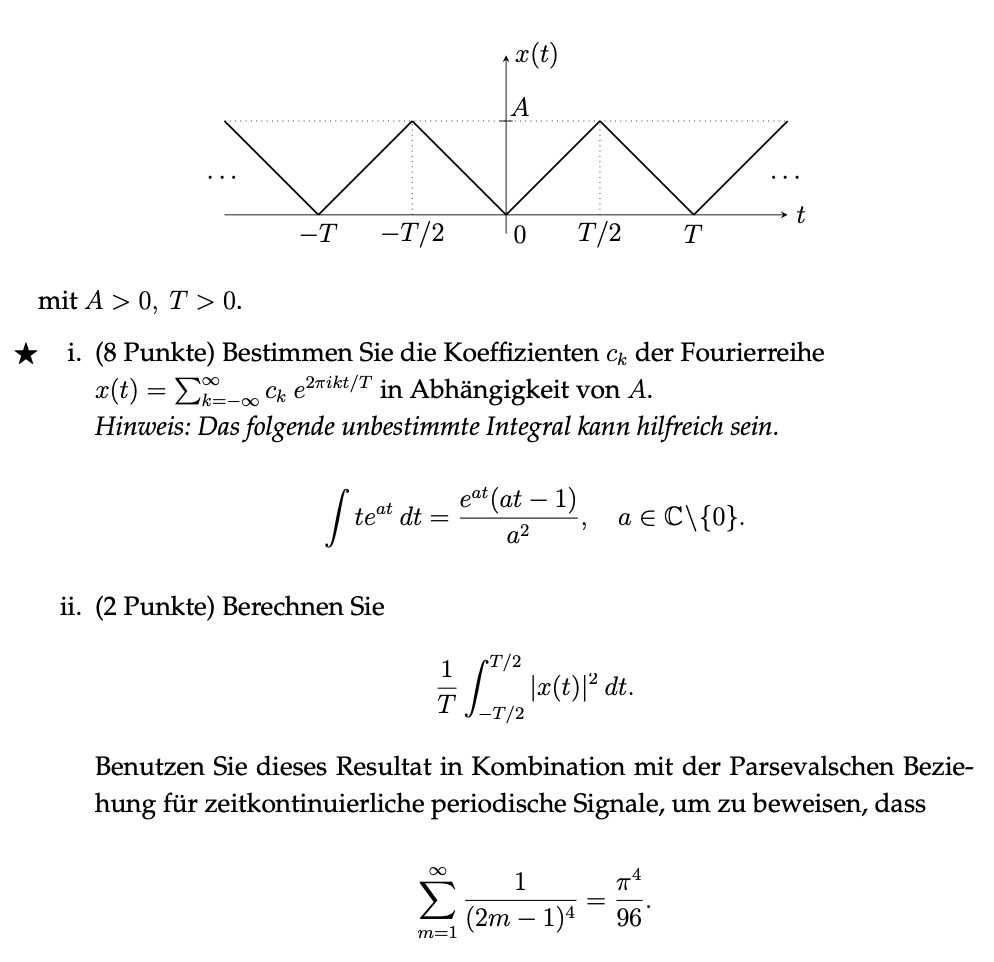
\includegraphics[width=0.9\linewidth]{docimgs/2024_ex1d_2.png}

\vfill \null
\pagebreak


\begin{tikzpicture}
    % Define the box size and grid spacing
    \draw[step=0.5cm,gray!50,very thin] (0,0) grid (16.5,21
    ); % (0,0) is bottom-left corner, (10,10) is top-right corner
\end{tikzpicture}

\pagebreak


\begin{tikzpicture}
    % Define the box size and grid spacing
    \draw[step=0.5cm,gray!50,very thin] (0,0) grid (16.5,21
    ); % (0,0) is bottom-left corner, (10,10) is top-right corner
\end{tikzpicture}

\pagebreak


\section*{Anwendung der Fouriertransformation auf LTI-Systeme}
\vspace*{-0.5cm}
\subsection*{Verzerrungsfreie Systeme}
\vspace*{-0.5cm}
\begin{center}
    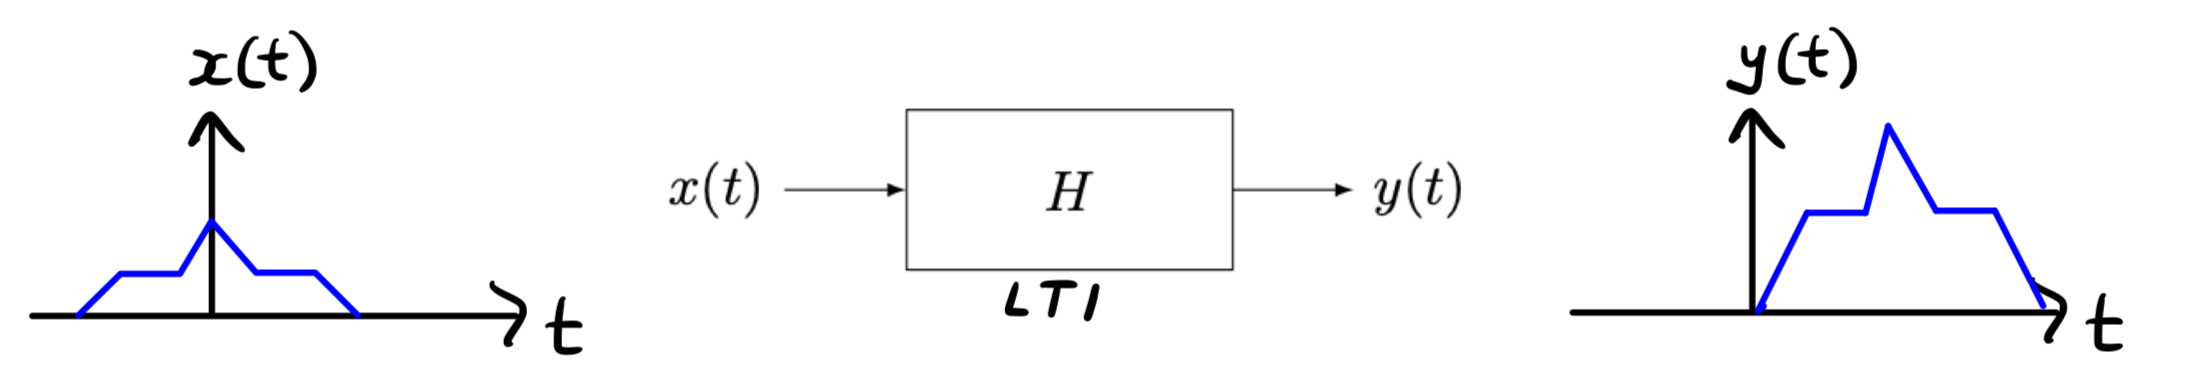
\includegraphics[width=0.8\linewidth]{docimgs/Verzerrungsfrei.jpg}
\end{center}
\vspace*{-0.5cm}
\textbf{Definition}: Ein \textbf{verzerrungsfreies} System hat folgende Eigenschaften:
\vspace*{-0.5cm}
\begin{enumerate}
    \item Input und Output haben die gleiche Form, d.h.\\
    $y(t) = kx(t-t_0) \; \transform{2.}{1.5} \; \hat{y}(f) = \underbrace{ke^{-2\pi i f t_0}}_{= \hat{h}(f)}\hat{x}(f)$
    \item $\hat{h}(f) = |\hat{h}(f)|e^{i \varphi(f)} = k e^{i(-2 \pi f t_0)} \; \invtransform{}{1.5} \; h(t) = k \delta(t-t_0)$
    \item Das System ist linear, stabil, kausal und zeitinvariant
\end{enumerate}
\vspace*{-0.5cm}
\begin{itemize}
    \item Verzerrungsfreie Systeme sind \textbf{Allpässe}, d.h. alle Frequenzen der Eingangssignale werden durchgelassen. Oft ist es jedoch nützlich, wenn wir bestimmte Frequenzen herausfiltern können. Dies entspricht einer Verzerrung des Eingangssignals.
    \item Ein Anwendungsgebiet wäre zum Beispiel, wenn wir aus einem Audiosignal hochfrequentes Rauschen (noise) rausfiltern möchten. In diesem Fall wollen wir, dass nur die tiefen Frequenzen des Eingangssignals durchgelassen werden. Das nennt man einen Tiefpassfilter.
\end{itemize}

\vspace*{-0.75cm}
\subsection*{Beispiel eines Tiefpassfilters}
\vspace*{-0.5cm}
\begin{center}
    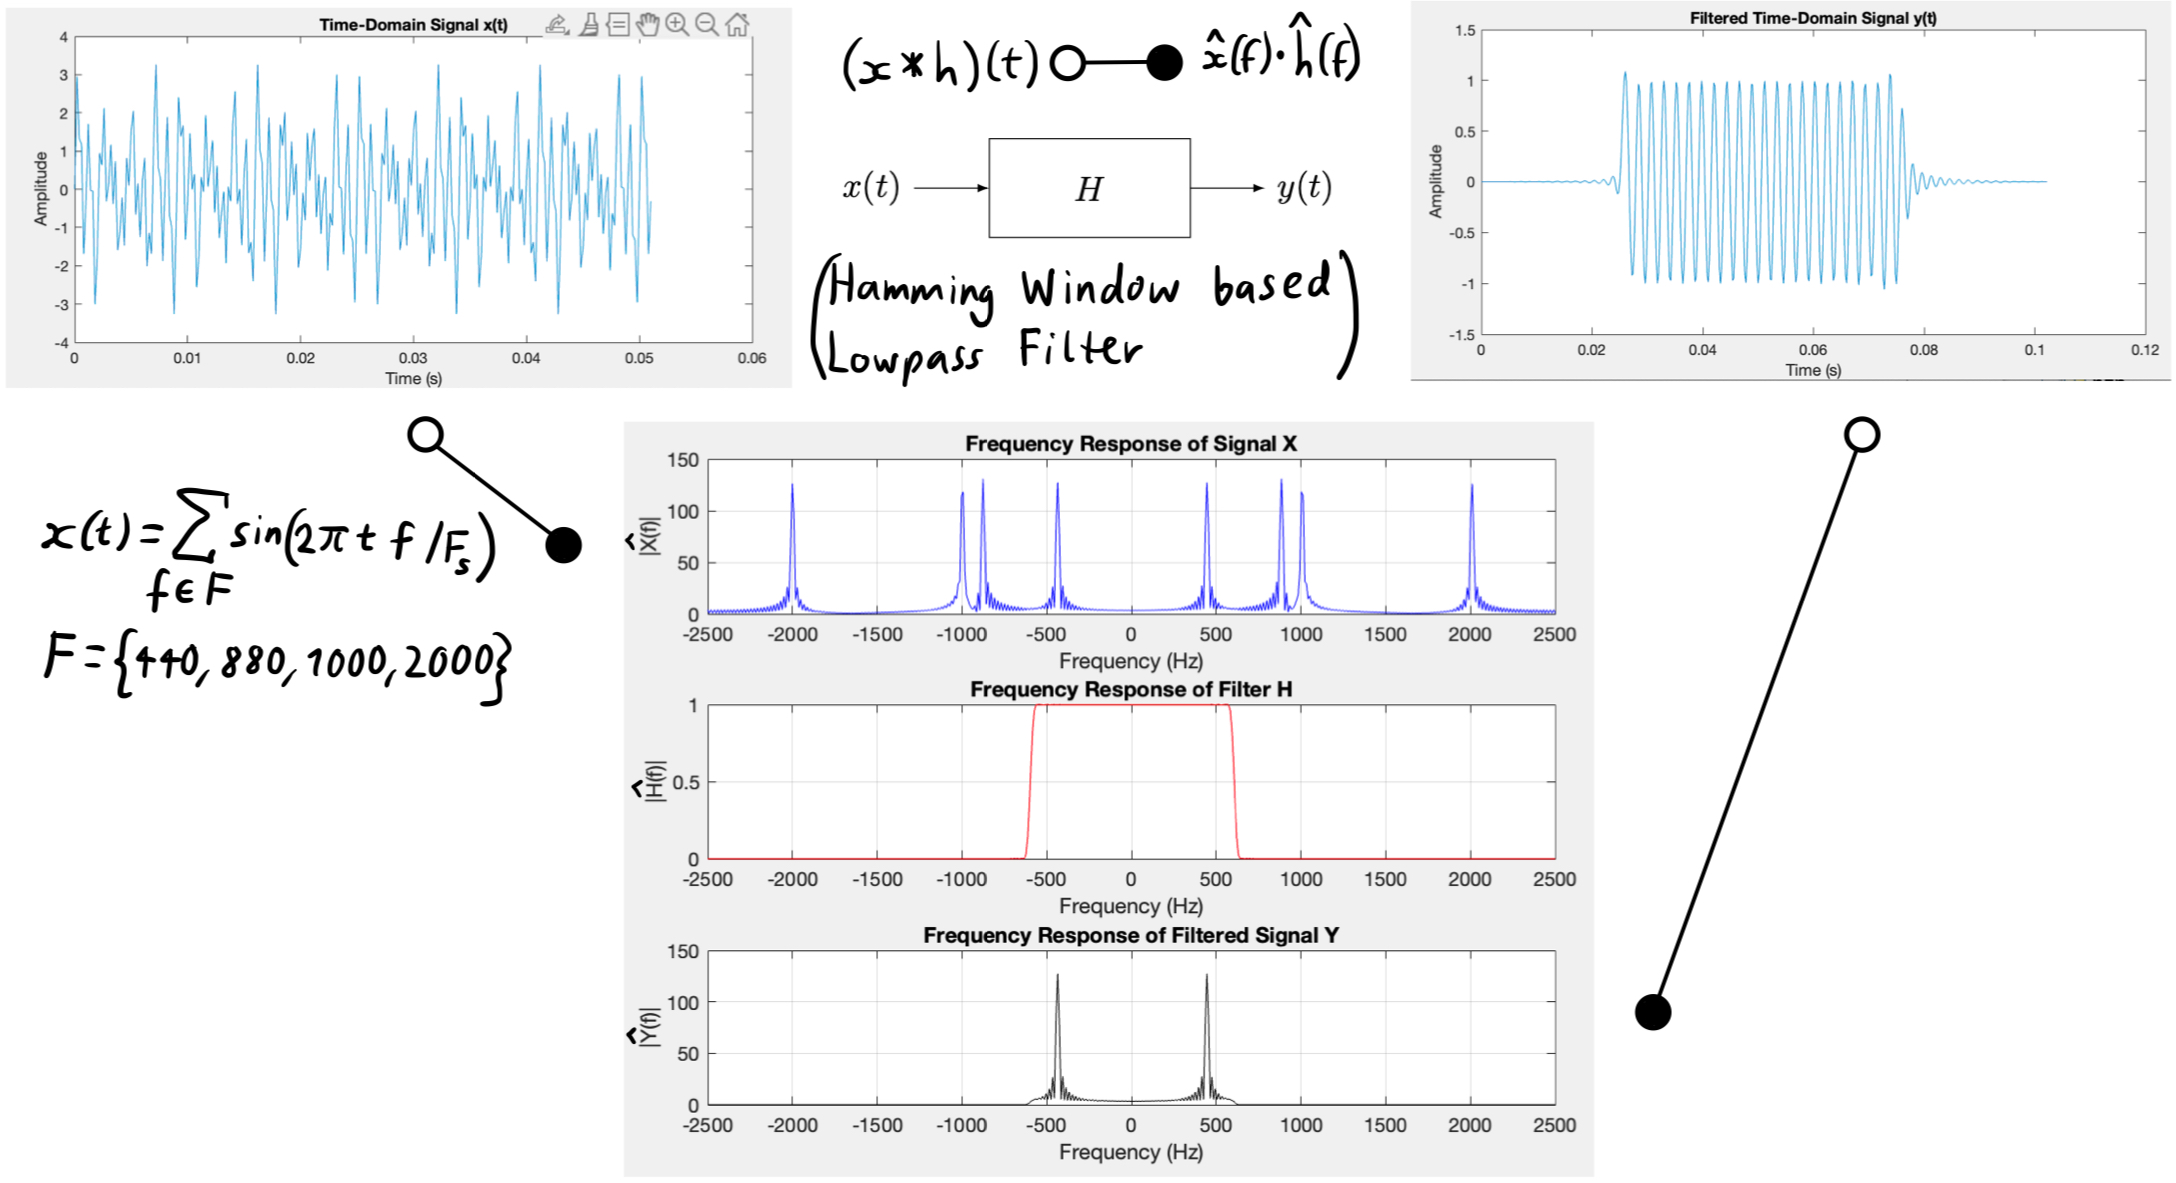
\includegraphics[width=0.9\linewidth]{docimgs/Hamming_lp.jpg}
\end{center}

\pagebreak
\subsection*{Idealisierte Tiefpassfilter}
\vspace*{-0.5cm}
\begin{center}
    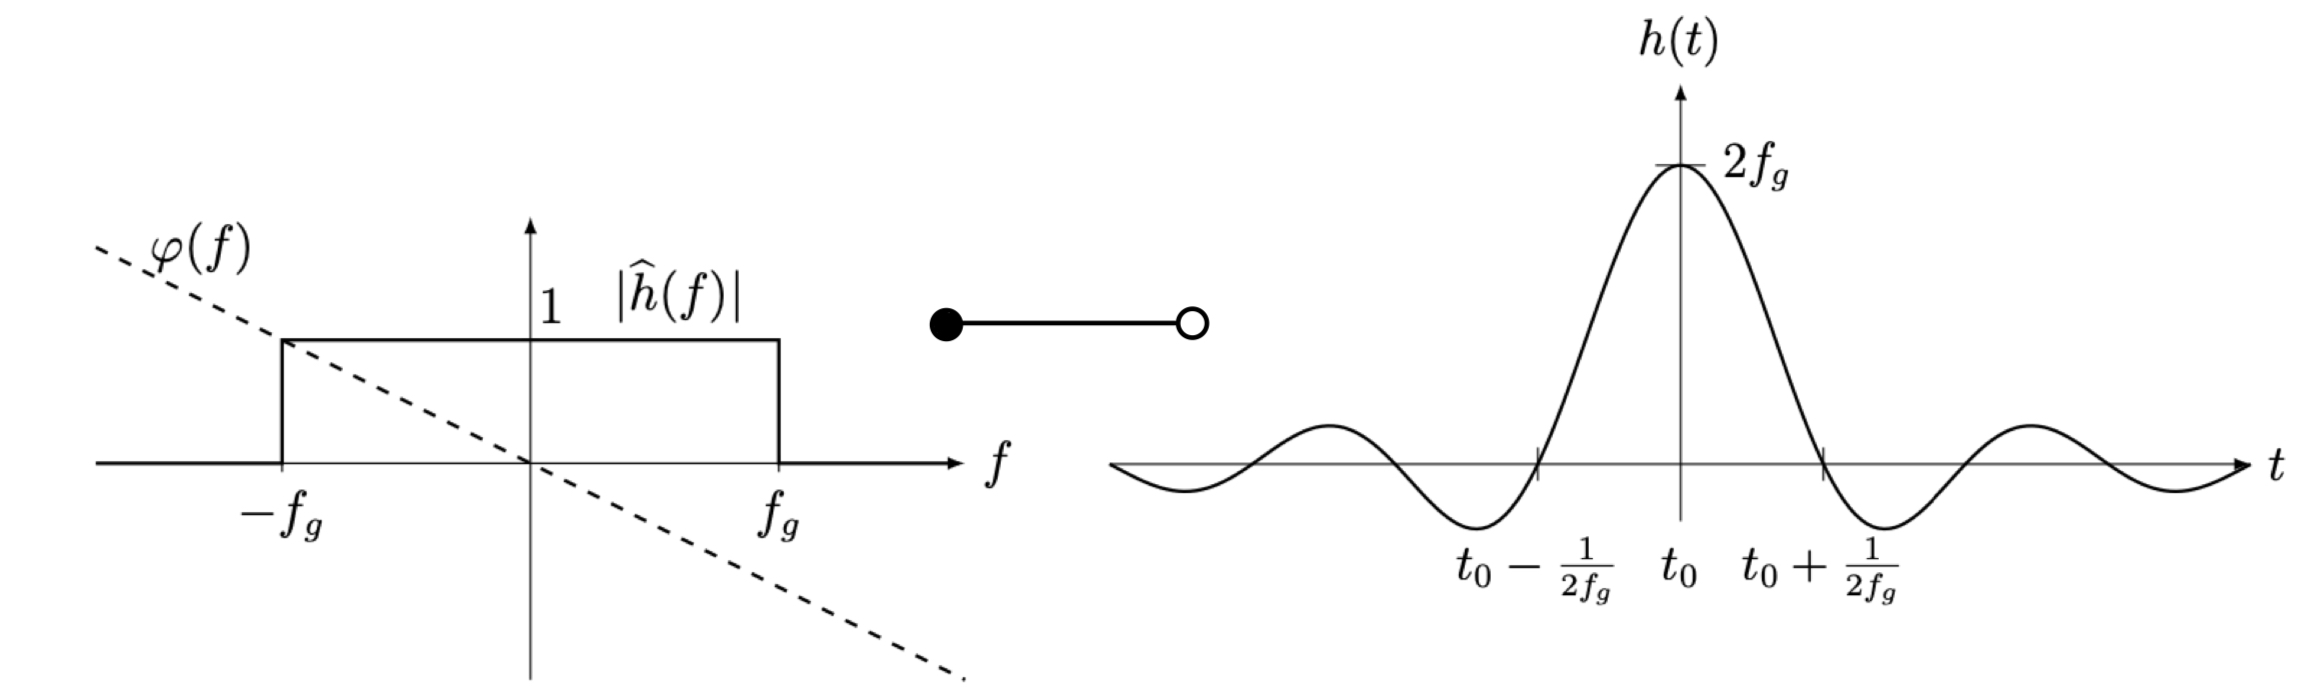
\includegraphics[width=0.8\linewidth]{docimgs/h_id.jpg}
\end{center}
\vspace*{-0.75cm}
Dieses System heisst Tiefpassfilter, da alle Frequenzen ausserhalb des Durchlassbereiches $[-f_g, f_g]$ aus dem Eingangssignal herausgefiltert werden. Ein ideales Tiefpassfilter ist mathematisch wie folgt beschrieben:
$$\hat{h}(f) = |\hat{h}(f)|e^{i \varphi(f)}, \hspace{12pt} \text{wobei} \hspace{12pt} |\hat{h}(f)|= \begin{cases}
    1, \; |f| \leq f_g\\
    0, \; \text{sonst}
\end{cases}, \hspace{12pt} \varphi(f) = -2 \pi f t_0$$
\begin{itemize}[leftmargin=0pt]
    \item[] $e^{i\varphi(f)}$ entspricht einer Zeitverzögerung von $t_0$.
    \item[] Wir schreiben $h(t) = \underbrace{|\hat{h}(f)|}_{=:\hat{h}_{id}(f)} e^{-2\pi i f t_0} \; \invtransform{2.}{1.5} \; h_{id}(t-t_0)$
    \item[] Aus FS. 27 erhalten wir, dass $h_{id}(t) = \displaystyle\frac{\sin(2 \pi f_g t)}{\pi t} \; \transform{27.}{1.5} \; \hat{h}_{id}(f) = \displaystyle\begin{cases}
        1, |f| \leq f_g\\
        0, \; \text{sonst}
    \end{cases}$ 
    \item[] Somit erhalten wir $h(t) = h_{id}(t-t_0) = \displaystyle\frac{\sin(2 \pi f_g (t-t_0))}{\pi (t-t_0)}$
\end{itemize}
\vspace*{-0.5cm}
\subsubsection*{Wichtige Bemerkungen}
\begin{enumerate}
    \item Da $h(t) = 0 \; \forall t < 0$ \textbf{nicht gilt}, ist das ideale Tiefpassfilter \textcolor{red}{\textbf{nicht kausal}}.
    \item Es gilt \textbf{nicht}, dass $\displaystyle\int_{-\infty}^{\infty} |h(t)|\text{d}t < \infty$, d.h. die Impulsantwort ist nicht absolut integrierbar. Somit ist das ideale Tiefpassfilter \textcolor{red}{\textbf{nicht BIBO-stabil}}.
    \item[] Der Grund hierfür liegt im Riemann-Lebesgue Lemma, das besagt, dass wenn das Signal $x$ absolut integrierbar ist, dann ist $(\mathcal{F}x)(f) = \hat{x}(f)$ stetig und es gilt $\displaystyle\lim_{|f|\to \infty}(\mathcal{F}x)(f)=0$.
    \item[] Da nun $\hat{h}(f)$ nicht stetig ist $\implies h(t)$ nicht absolut integrierbar.
    \item[1.\&2.] $\implies$ Ideale Tiefpassfilter sind \textcolor{red}{\textbf{nicht realisierbar}} in der Praxis. Wir müssen das Filter kausal und BIBO-stabil machen!
\end{enumerate}

\pagebreak

\subsubsection*{Kausalisierung}
\vspace*{-0.5cm}
\begin{itemize}[leftmargin = 0pt]
    \item[] Da das System LTI ist, wollen wir um Kausalität zu erreichen $h(t) = 0 \; \forall t < 0$ haben.
    \item[] Im Zeitbereich: $h_{id}(t) = \displaystyle\frac{\sin(2 \pi f_g t)}{\pi t}$
    \item[] Nun verschieben wir $h_{id}(t)$ um $t_1$ und multiplizieren das verschobene ideale Tiefpassfilter mit der Einheitssprungfunktion $\sigma(t)$. So erhalten wir $h(t) = 0 \; \forall t < 0$.
    \item[] Somit $h_{kaus}(t) = h_{id}(t-t_1)\sigma(t)$
    \item[] \begin{center}
        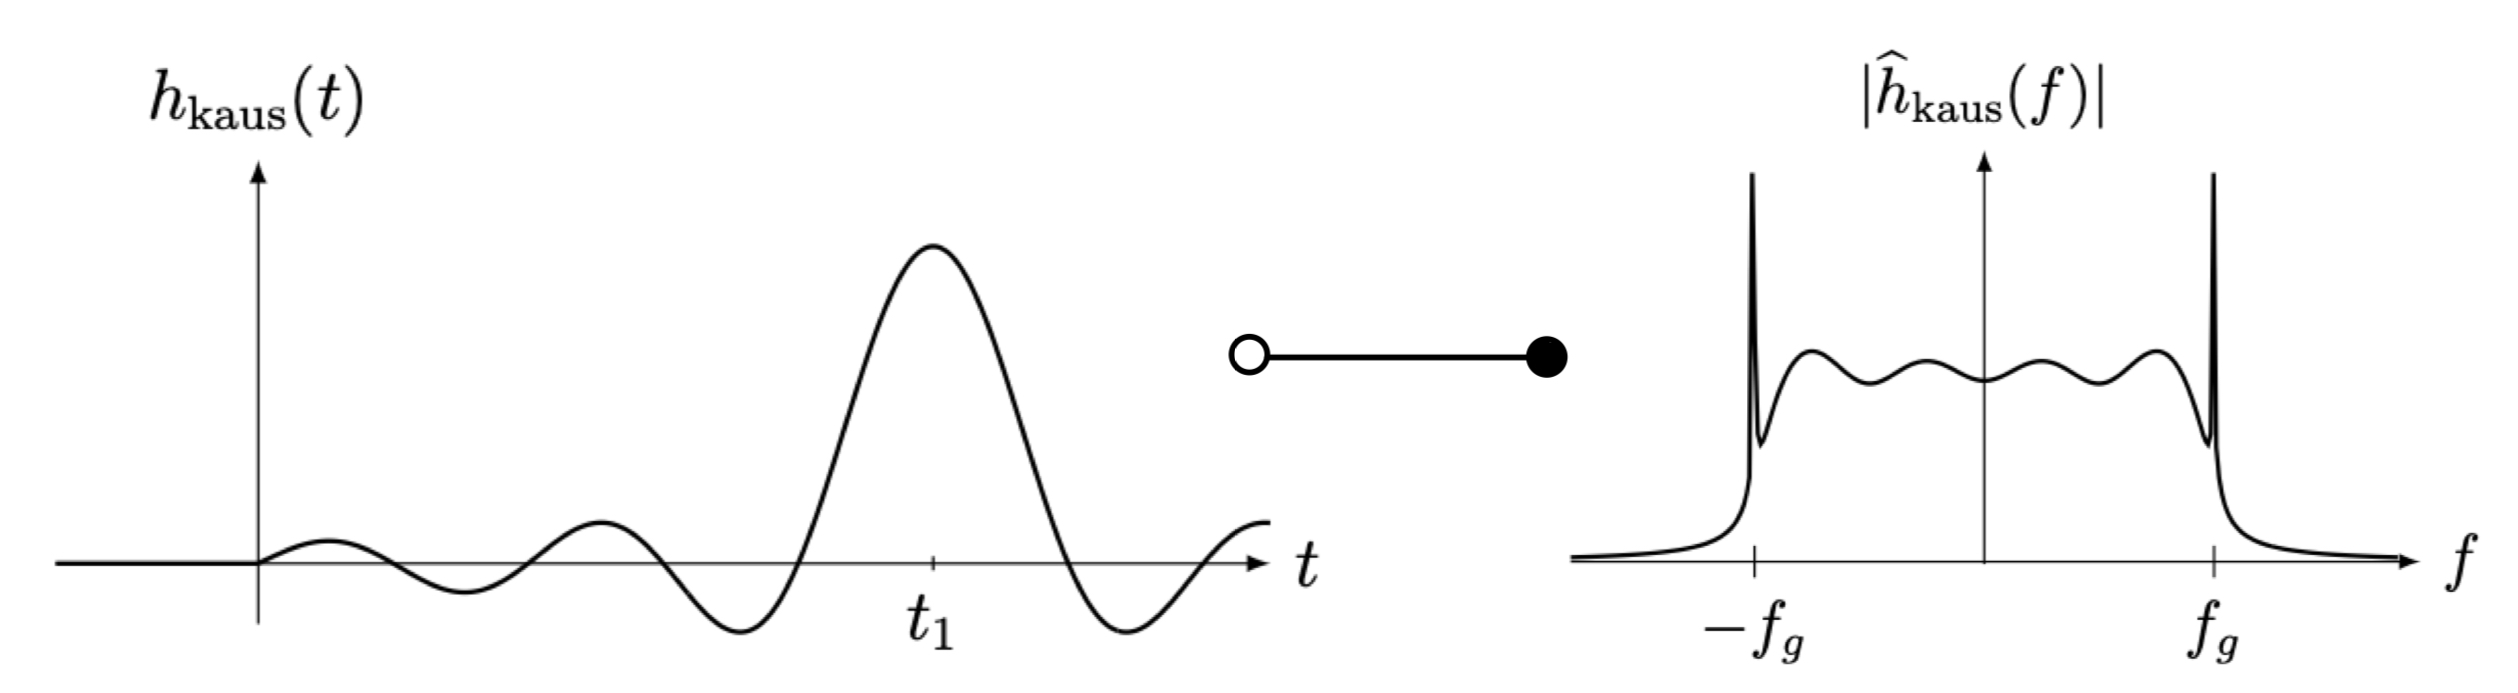
\includegraphics[width=0.8\linewidth]{docimgs/h_kausal.jpg}
    \end{center}
    \item[] Wenn wir die dazugehörige Fouriertransformation $\hat{h}_{kaus}(f)$ bestimmen, dann sehen wir, dass die Frequenzen bei $\pm f_g$ deutlich verstärkt werden. Somit ist $h_{kaus}$ kein gutes Filter.
\end{itemize}

\vspace*{-0.5cm}
\subsubsection*{Stabilisierung}
\vspace*{-0.5cm}
\begin{itemize}[leftmargin=0pt]
    \item[] Wir wollen $h(t) \in L^1$ (absolut integrierbar). Aus diesem Grund falten wir $\hat{h}_{id}(f)$ mit $\hat{h}_{ge}(f)$.
    \item[] \begin{center}
        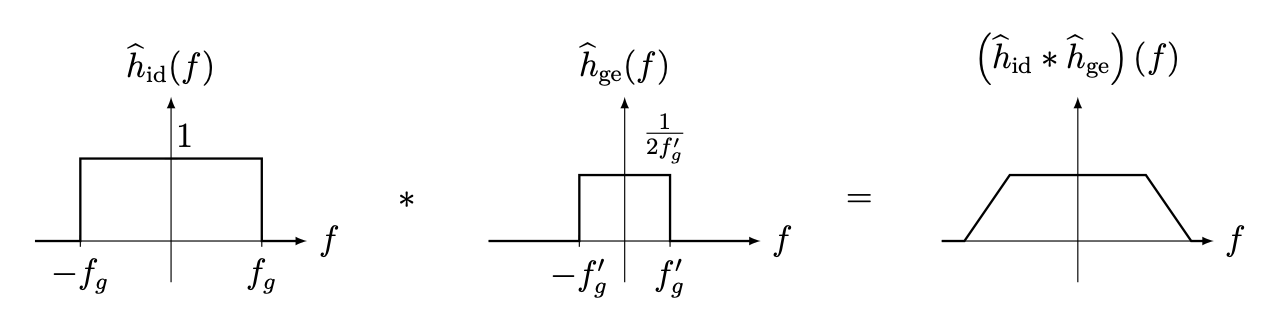
\includegraphics[width=0.7\linewidth]{docimgs/h_stabil_freq.png}
    \end{center}
    \item[] Somit erhalten wir $(\hat{h}_{id} \ast \hat{h}_{ge})(f) \; \invtransform{}{1.5} \; h_{id}(t) h_{ge}(t) \propto \displaystyle\frac{1}{t} \cdot \displaystyle\frac{1}{t} = \displaystyle\frac{1}{t^2} \in L^1$
    \item[] Das resultierende Tiefpassfilter ist BIBO-stabil und sieht im Frequenzbereich aus wie folgt:
    \item[] \begin{center}
        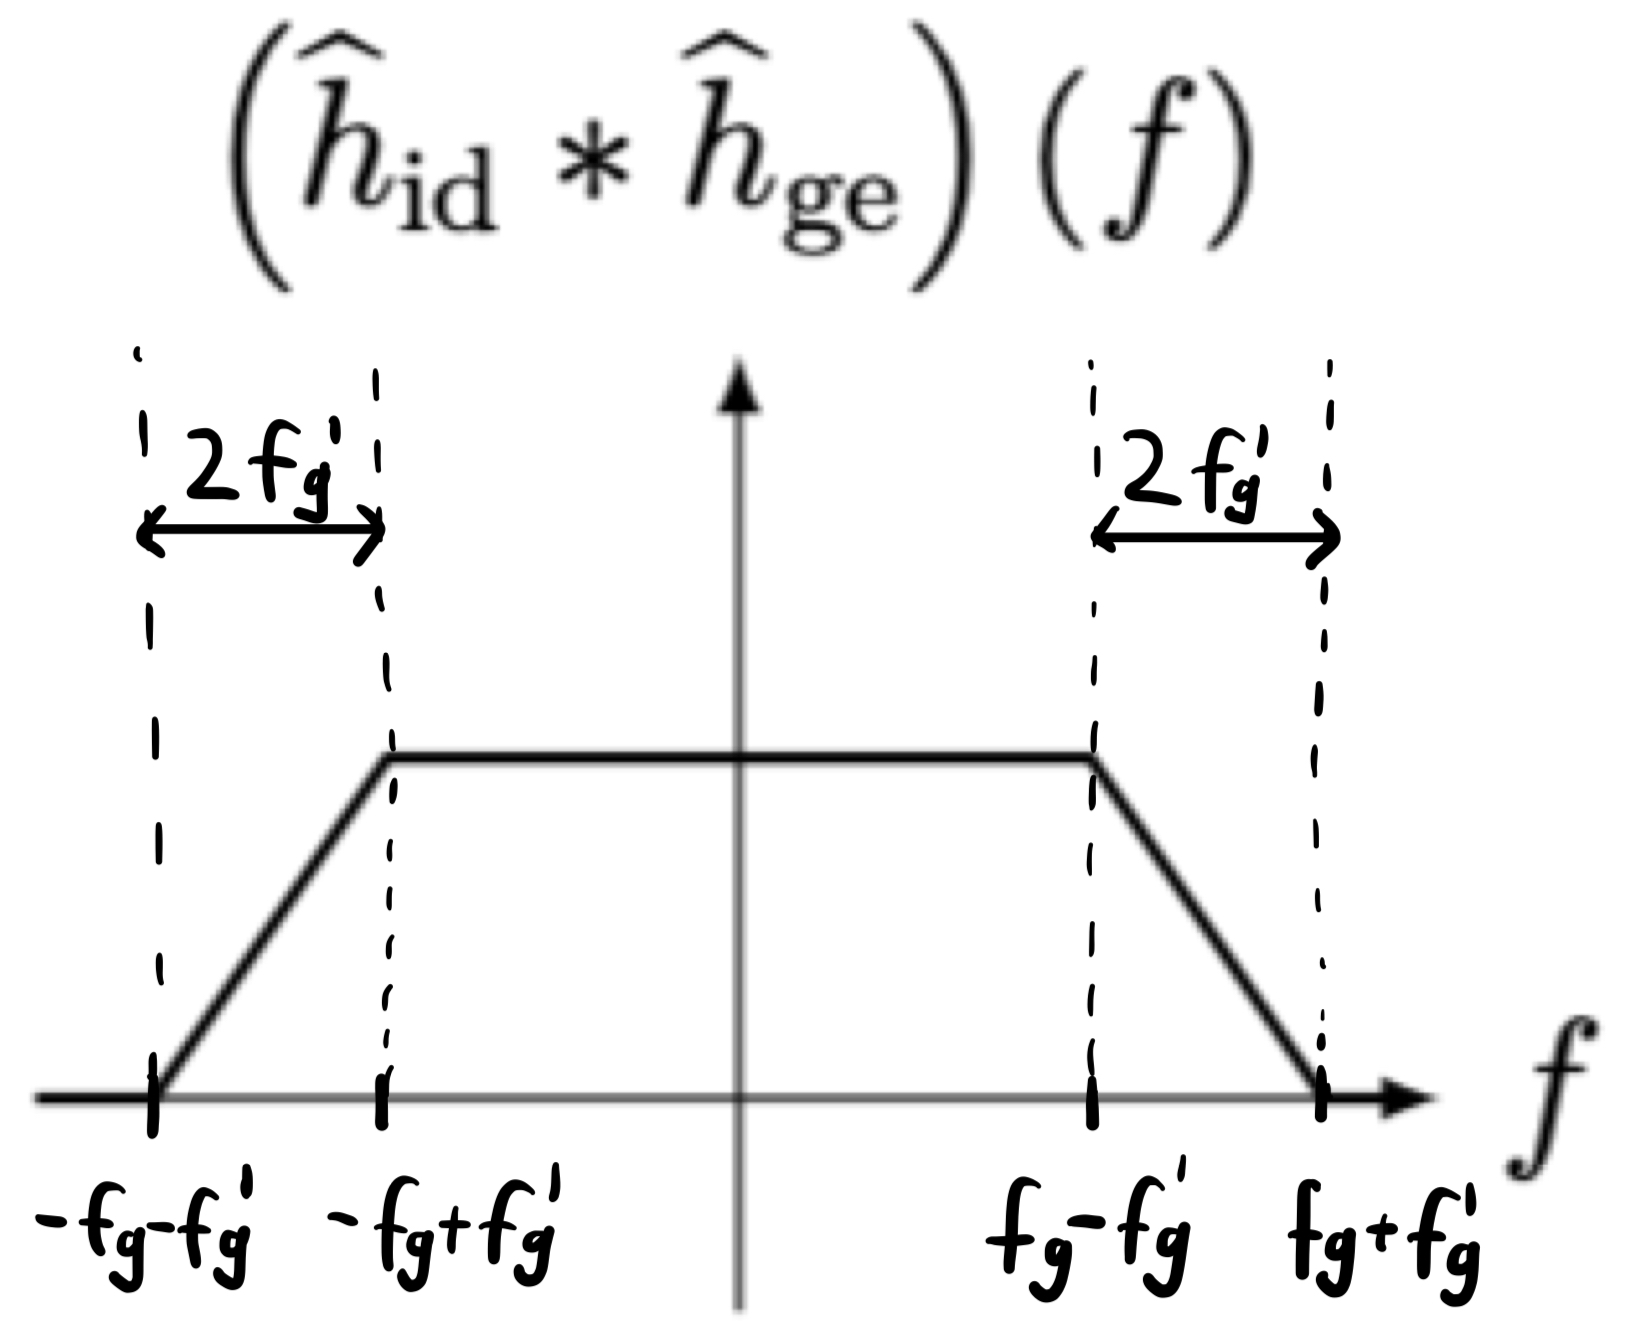
\includegraphics[width=0.2\linewidth]{docimgs/h_stabil_2.jpg}
    \end{center}
    \item[] Da dieses Filter nicht perfekt ist in den Bereichen $|f \pm f_g| \in [-f_g', f_g']$, versucht man $f_g'$ so klein wie möglich zu wählen.
\end{itemize}

\pagebreak

\subsection*{Bandbegrenzte Signale}
\vspace*{-0.5cm}
\begin{itemize}[leftmargin=0pt]
    \item[] \textbf{Definition}: Die \textbf{Bandbreite} des Signals $x$ ist das kleinste $W$, so dass
    $$(x \ast h_{\text{TP,}W})(t) = x(t), \hspace{12pt} \text{für alle } t \in \mathbb{R}, \text{ wobei}$$
    $$h_{\text{TP,}W}(t) = \sin (2 \pi W t)/(\pi t).$$
    \item[] Im Frequenzbereich bedeutet das
    $$\hat{x}(f)\hat{h}_{\text{TP,}W}(f) = \hat{x}(f), \hspace{12pt} \text{für alle }f\in \mathbb{R}, \text{ und}$$
    $$\hat{h}_{\text{TP,}W}(f) = \begin{cases}
        1, \; |f| \leq W \\
        0, \; \text{sonst.}
    \end{cases}$$
    \item[] \textbf{Intuitiv} bedeutet diese Definition das folgende: Die Bandbreite ist die betragsweise höchste Frequenz (positiv oder negativ), die in einem Signal enthalten ist.
    \item[] \textbf{Beispiele}:
    \item[] \begin{center}
        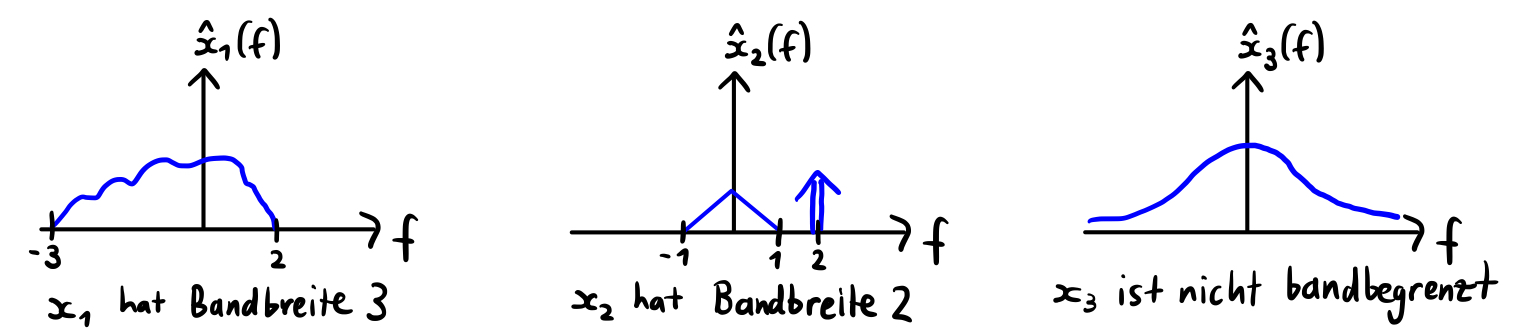
\includegraphics[width=0.9\linewidth]{docimgs/Bandbreite.jpg}
    \end{center}
    \item[] \textbf{Bemerkung}: Seien $x_1, x_2$ zwei Signale mit Bandbreite $W_1$ resp. $W_2$ \begin{itemize}
        \item $x_1(t) + x_2(t)$ hat Bandbreite max$\{W_1, W_2\}$
        \item $(x_1 \ast x_2)(t)$ hat Bandbreite min$\{W_1, W_2\}$
        \item $x_1(t)x_2(t)$ hat Bandbreite $\leq W_1 + W_2$
    \end{itemize}
\end{itemize}

\vspace*{-0.5cm}
\subsubsection*{Bernstein'sche Ungleichung}
\vspace*{-0.5cm}
\textbf{Theorem}: Wenn $x(t)$ in der Form $$x(t) = \displaystyle\int_{-W}^W g(f)e^{2 \pi i f t} \text{d}f, \text{ für alle } t\in \mathbb{R}$$ dargestellt werden kann, für eine integrierbare Funktion $g$, d.h. $g\in L^1$, dann gilt $$\left| \frac{\text{d}x(t)}{\text{d}t} \right| \leq 4 \pi W \sup_{\tau \in \mathbb{R}}|x(t)|, \hspace{12pt} \text{für alle } t \in \mathbb{R}.$$

\begin{itemize}[leftmargin=0pt]
    \item[] Dieses Kriterium liefert uns eine Abschätzung für die Ableitung von $x(t)$.
    \item[] Eine kleine Bandbreite $W \implies$ nur tiefe Frequenzen sind im Signal enthalten $\implies x(t)$ kann sich nur "langsam" ändern.
\end{itemize}

\pagebreak

\subsection*{Aufgabe 68}
\vspace*{-0.5cm}
Das Signal $x(t)$ habe die Bandbreite $f_0$, d.h. $\hat{x}(f) = 0$ für $|f|>f_0$. Bestimmen Sie die Bandbreiten der folgenden Signale in Abhängigkeit von $f_0$.
\begin{multicols}{2}
    \begin{itemize}
        \item[a)] $x(t) + x(t-1)$
        \item[b)] $\displaystyle\frac{\text{d}x(t)}{\text{d}t}$
        \item[c)] $x^2(t)$
        \item[d)] $x(t)\cos(2 \pi f_0 t)$
    \end{itemize}
\end{multicols}


\begin{tikzpicture}
    % Define the box size and grid spacing
    \draw[step=0.5cm,gray!50,very thin] (0,0) grid (16.5,16
    ); % (0,0) is bottom-left corner, (10,10) is top-right corner
\end{tikzpicture}

\end{document}